% Practice Test 12 — Virginia Edition
% Questions: 30 (17 MC + 13 SA)
% Generated by scripts/generate_practice_tests.py

\begin{practiceQuestion}{1-4-q20}{sa}
\begin{questionText}
Using the equation $y = 3.5x$, find $y$ when $x = 14$.
\end{questionText}
\correctAnswer{$y = 49$}
\explanation{$y = 3.5 \times 14 = 49$.}
\end{practiceQuestion}

\begin{practiceQuestion}{2-1-q20}{sa}
\begin{questionText}
$42$ is what percent of $168$?
\end{questionText}
\correctAnswer{$25\%$}
\explanation{Divide the part by the whole: $42 \div 168 = 0.25 = 25\%$.}
\end{practiceQuestion}

\begin{practiceQuestion}{2-2-q19}{sa}
\begin{questionText}
Use a proportion to find $85\%$ of $260$.
\end{questionText}
\correctAnswer{$221$}
\explanation{$\frac{n}{260} = \frac{85}{100}$. Cross-multiply: $100n = 22{,}100$. Divide: $n = 221$.}
\end{practiceQuestion}

\begin{practiceQuestion}{2-3-q21}{sa}
\begin{questionText}
What multiplier represents a $5\%$ increase?
\end{questionText}
\correctAnswer{$1.05$}
\explanation{$1 + 0.05 = 1.05$.}
\end{practiceQuestion}

\begin{practiceQuestion}{2-7-q10}{mc}
\begin{questionText}
A weather forecast predicted $3$ inches of rain. The actual rainfall was $2.5$ inches. What is the percent error?
\end{questionText}
\choiceA{$0.5\%$}
\choiceB{$10\%$}
\choiceC{$16.7\%$}
\choiceD{$20\%$}
\correctAnswer{D}
\explanation{$\frac{|3 - 2.5|}{2.5} \times 100 = \frac{0.5}{2.5} \times 100 = 20\%$.}
\end{practiceQuestion}

\begin{practiceQuestion}{3-2-q29}{gsa}
\begin{questionText}
The number line shows two jumps. Write the addition sentence and find the final position.

\begin{center}
\begin{tikzpicture}
  \draw[thick,->] (-8.5,0) -- (4.5,0);
  \foreach \x in {-8,...,4} \draw (\x,0.1) -- (\x,-0.1) node[below] {\footnotesize $\x$};
  \fill[black] (2,0) circle (3pt);
  \draw[thick,->,funBlue] (2,0.5) -- (-3,0.5);
  \node[above,funBlue] at (-0.5,0.5) {$-5$};
  \draw[thick,->,funRed] (-3,0.9) -- (-7,0.9);
  \node[above,funRed] at (-5,0.9) {$-4$};
\end{tikzpicture}
\end{center}
\end{questionText}
\correctAnswer{$2 + (-5) + (-4) = -7$}
\explanation{Start at $2$, move $5$ left to $-3$, then $4$ more left to $-7$. The expression is $2 + (-5) + (-4) = -7$.}
\end{practiceQuestion}

\begin{practiceQuestion}{3-3-q23}{sa}
\begin{questionText}
What is $(-6) - (-6) - 6$?
\end{questionText}
\correctAnswer{$-6$}
\explanation{$(-6) - (-6) = (-6) + 6 = 0$. Then $0 - 6 = -6$.}
\end{practiceQuestion}

\begin{practiceQuestion}{3-4-q27}{gmc}
\begin{questionText}
The fraction bars below compare two quantities.

\begin{center}
\begin{tikzpicture}
  % First bar: -3/4
  \node[left] at (0,1.2) {$-\dfrac{3}{4}$:};
  \draw[thick] (1,1) rectangle (5,1.4);
  \fill[funRed!40] (1,1) rectangle (4,1.4);
  \node at (2.5,1.2) {\footnotesize shaded};
  % Second bar: +1/4
  \node[left] at (0,0.2) {$+\dfrac{1}{4}$:};
  \draw[thick] (1,0) rectangle (5,0.4);
  \fill[funBlue!40] (1,0) rectangle (2,0.4);
  \node at (1.5,0.2) {\footnotesize shaded};
\end{tikzpicture}
\end{center}

What is $-\dfrac{3}{4} + \dfrac{1}{4}$?
\end{questionText}
\choiceA{$-1$}
\choiceB{$-\dfrac{1}{2}$}
\choiceC{$\dfrac{1}{2}$}
\choiceD{$1$}
\correctAnswer{B}
\explanation{$-\frac{3}{4} + \frac{1}{4} = -\frac{2}{4} = -\frac{1}{2}$. Different signs: $3 - 1 = 2$ fourths, keep negative.}
\end{practiceQuestion}

\begin{practiceQuestion}{4-3-q20}{sa}
\begin{questionText}
Expand and simplify $3(2x + 4) - 5x$.
\end{questionText}
\correctAnswer{$x + 12$}
\explanation{Expand: $6x + 12$. Subtract $5x$: $6x + 12 - 5x = x + 12$.}
\end{practiceQuestion}

\begin{practiceQuestion}{4-4-q10}{mc}
\begin{questionText}
Factor $18a + 12b + 6$.
\end{questionText}
\choiceA{$6(3a + 2b + 1)$}
\choiceB{$3(6a + 4b + 2)$}
\choiceC{$2(9a + 6b + 3)$}
\choiceD{$6(3a + 2b + 6)$}
\correctAnswer{A}
\explanation{GCF of $18$, $12$, and $6$ is $6$. Divide each: $18a \div 6 = 3a$, $12b \div 6 = 2b$, $6 \div 6 = 1$. Result: $6(3a + 2b + 1)$.}
\end{practiceQuestion}

\begin{practiceQuestion}{5-4-q24}{sa}
\begin{questionText}
Solve $\dfrac{5n}{6} + \dfrac{1}{3} = 3$.
\end{questionText}
\correctAnswer{$n = \dfrac{16}{5}$ or $3\dfrac{1}{5}$}
\explanation{Multiply every term by $6$: $5n + 2 = 18$. Subtract $2$: $5n = 16$. Divide by $5$: $n = \frac{16}{5} = 3\frac{1}{5}$.}
\end{practiceQuestion}

\begin{practiceQuestion}{5-5-q15}{mc}
\begin{questionText}
A student needs at least $70$ points to pass a test. She earns $4$ points per question and has $10$ bonus points. Which inequality finds the minimum number of questions $q$ she must answer?
\end{questionText}
\choiceA{$4q + 10 > 70$}
\choiceB{$4q + 10 \geq 70$}
\choiceC{$4q - 10 \geq 70$}
\choiceD{$10q + 4 \geq 70$}
\correctAnswer{B}
\explanation{Score $= 4q + 10$, needs at least $70$: $4q + 10 \geq 70$.}
\end{practiceQuestion}

\begin{practiceQuestion}{5-6-q03}{mc}
\begin{questionText}
Solve $x + 5 \geq 9$ and choose the correct graph description.
\end{questionText}
\choiceA{Closed circle at $4$, shade right}
\choiceB{Open circle at $4$, shade right}
\choiceC{Closed circle at $4$, shade left}
\choiceD{Open circle at $14$, shade right}
\correctAnswer{A}
\explanation{Subtract $5$: $x \geq 4$. Closed circle at $4$ (includes $4$), shade right.}
\end{practiceQuestion}

\begin{practiceQuestion}{6-1-q16}{mc}
\begin{questionText}
A blueprint has a scale of $1$ in $= 12$ ft. A wall is $4\frac{1}{4}$ in on the blueprint. What is the actual length of the wall?
\end{questionText}
\choiceA{$48$ ft}
\choiceB{$49$ ft}
\choiceC{$51$ ft}
\choiceD{$16.25$ ft}
\correctAnswer{C}
\explanation{$4\frac{1}{4} = 4.25$. Multiply: $4.25 \times 12 = 51$ ft.}
\end{practiceQuestion}

\begin{practiceQuestion}{6-2-q09}{mc}
\begin{questionText}
A map uses $1$ cm $= 40$ km. A lake is $3$ cm wide on this map. You redraw the map at $1$ cm $= 8$ km. How wide is the lake on the new map?
\end{questionText}
\choiceA{$0.6$ cm}
\choiceB{$5$ cm}
\choiceC{$15$ cm}
\choiceD{$24$ cm}
\correctAnswer{C}
\explanation{Scale ratio: $\frac{40}{8} = 5$. New width: $3 \times 5 = 15$ cm.}
\end{practiceQuestion}

\begin{practiceQuestion}{6-5-q27}{gmc}
\begin{questionText}
The diagram shows a cone being sliced. Which cut produces a circular cross-section?

\begin{center}
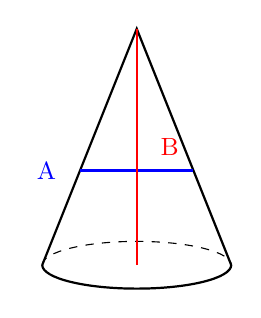
\begin{tikzpicture}[scale=0.6]
  % Cone
  \draw[thick] (-2,0) -- (0,5) -- (2,0);
  \draw[thick] (-2,0) arc[start angle=180,end angle=360,x radius=2,y radius=0.5];
  \draw[dashed] (-2,0) arc[start angle=180,end angle=0,x radius=2,y radius=0.5];
  % Cut A - horizontal
  \draw[thick,blue] (-1.2,2) -- (1.2,2);
  \node[left,blue] at (-1.5,2) {\small A};
  % Cut B - vertical through apex
  \draw[thick,red] (0,0) -- (0,5);
  \node[right,red] at (0.3,2.5) {\small B};
\end{tikzpicture}
\end{center}
\end{questionText}
\choiceA{Cut A (horizontal)}
\choiceB{Cut B (vertical through apex)}
\choiceC{Both cuts}
\choiceD{Neither cut}
\correctAnswer{A}
\explanation{Cut A (horizontal, parallel to the base) produces a circle. Cut B (vertical through the apex) produces a triangle.}
\end{practiceQuestion}

\begin{practiceQuestion}{6-6-q15}{mc}
\begin{questionText}
Which pair of angles is complementary?
\end{questionText}
\choiceA{$50°$ and $130°$}
\choiceB{$55°$ and $35°$}
\choiceC{$60°$ and $60°$}
\choiceD{$45°$ and $135°$}
\correctAnswer{B}
\explanation{Complementary angles sum to $90°$. Only $55 + 35 = 90$.}
\end{practiceQuestion}

\begin{practiceQuestion}{6-7-q02}{mc}
\begin{questionText}
Point $B(-2, 4)$ is reflected over the $x$-axis. What are the coordinates of $B'$?
\end{questionText}
\choiceA{$(-2, -4)$}
\choiceB{$(2, 4)$}
\choiceC{$(2, -4)$}
\choiceD{$(-2, 4)$}
\correctAnswer{A}
\explanation{Reflection over the $x$-axis: keep $x$, negate $y$. $(-2, 4) \to (-2, -4)$.}
\end{practiceQuestion}

\begin{practiceQuestion}{6-8-q23}{sa}
\begin{questionText}
A scale model of a bridge is $18$ inches long. The actual bridge is $900$ feet long. What is the scale factor (as a ratio of model to actual)?
\end{questionText}
\correctAnswer{$1:600$}
\explanation{Convert $900$ ft to inches: $900 \times 12 = 10{,}800$ inches. Scale: $\frac{18}{10{,}800} = \frac{1}{600}$. The ratio is $1:600$.}
\end{practiceQuestion}

\begin{practiceQuestion}{7-4-q24}{sa}
\begin{questionText}
A shape is made of two congruent triangles, each with base $8$ cm and height $5$ cm, joined along their bases. What is the total area?
\end{questionText}
\correctAnswer{$40$ cm$^2$}
\explanation{Each triangle: $\frac{1}{2} \times 8 \times 5 = 20$ cm$^2$. Two triangles: $20 + 20 = 40$ cm$^2$.}
\end{practiceQuestion}

\begin{practiceQuestion}{7-5-q28}{gmc}
\begin{questionText}
The diagram shows a triangular prism. What is its total surface area?

\begin{center}
\begin{tikzpicture}[scale=0.4]
  % Front triangle
  \draw[thick,funBlue,fill=funBlue!10] (0,0) -- (6,0) -- (3,4) -- cycle;
  % Back triangle (offset)
  \draw[thick,funBlue,fill=funBlue!20] (2,1.5) -- (8,1.5) -- (5,5.5) -- cycle;
  % Connecting edges
  \draw[thick,funBlue] (0,0) -- (2,1.5);
  \draw[thick,funBlue] (6,0) -- (8,1.5);
  \draw[thick,funBlue] (3,4) -- (5,5.5);
  % Labels
  \node[below] at (3,0) {$6$ cm};
  \node[left] at (1.2,2) {$5$ cm};
  \node[right] at (4.8,2) {$5$ cm};
  \node[right] at (8,3.5) {$8$ cm};
  \node[above left] at (1,0.8) {$h = 4$ cm};
\end{tikzpicture}
\end{center}
\end{questionText}
\choiceA{$104$ cm$^2$}
\choiceB{$128$ cm$^2$}
\choiceC{$152$ cm$^2$}
\choiceD{$160$ cm$^2$}
\correctAnswer{C}
\explanation{Two triangles: $2 \times \frac{1}{2} \times 6 \times 4 = 24$ cm$^2$. Three rectangles: $6 \times 8 + 5 \times 8 + 5 \times 8 = 48 + 40 + 40 = 128$ cm$^2$. Total: $24 + 128 = 152$ cm$^2$.}
\end{practiceQuestion}

\begin{practiceQuestion}{7-6-q05}{mc}
\begin{questionText}
A triangular prism has a base that is a triangle with base $8$ cm and height $3$ cm. The prism is $10$ cm long. What is the volume?
\end{questionText}
\choiceA{$24$ cm$^3$}
\choiceB{$80$ cm$^3$}
\choiceC{$120$ cm$^3$}
\choiceD{$240$ cm$^3$}
\correctAnswer{C}
\explanation{$B = \frac{1}{2} \times 8 \times 3 = 12$ cm$^2$. $V = Bh = 12 \times 10 = 120$ cm$^3$.}
\end{practiceQuestion}

\begin{practiceQuestion}{7-7-q30}{gsa}
\begin{questionText}
A cylindrical water bottle is shown. Find its volume. Use $\pi \approx 3.14$.

\begin{center}
\begin{tikzpicture}[scale=0.25]
  \draw[thick,funBlue,fill=cyan!10] (-2.5,0) -- (-2.5,14) arc (180:360:2.5 and 0.8) -- (2.5,0) arc (0:180:2.5 and 0.8);
  \draw[thick,funBlue,fill=cyan!20] (0,14) ellipse (2.5 and 0.8);
  \draw[thick,dashed,funBlue] (-2.5,0) arc (180:360:2.5 and 0.8);
  \draw[thick,funRed,<->] (4,0) -- (4,14);
  \node[right,funRed] at (4,7) {$20$ cm};
  \draw[thick,funRed,<->] (0,14) -- (2.5,14);
  \node[above,funRed] at (1.25,15) {$r = 3.5$ cm};
\end{tikzpicture}
\end{center}
\end{questionText}
\correctAnswer{$769.3$ cm$^3$}
\explanation{$V = \pi r^2 h = 3.14 \times (3.5)^2 \times 20 = 3.14 \times 12.25 \times 20 = 769.3$ cm$^3$.}
\end{practiceQuestion}

\begin{practiceQuestion}{8-1-q17}{mc}
\begin{questionText}
A doctor wants to study the effect of a new medicine on $10{,}000$ patients. She randomly selects $500$ patients for a trial. What is the sample size?
\end{questionText}
\choiceA{$10{,}000$}
\choiceB{$500$}
\choiceC{$10{,}500$}
\choiceD{$50$}
\correctAnswer{B}
\explanation{The sample size is the number of individuals selected — $500$ patients.}
\end{practiceQuestion}

\begin{practiceQuestion}{8-3-q07}{mc}
\begin{questionText}
Two box plots are drawn on the same number line. Box plot A is entirely to the right of box plot B. What does this tell you?
\end{questionText}
\choiceA{Group A has more data}
\choiceB{All values in Group A are greater than all values in Group B}
\choiceC{Group A has no overlap with Group B}
\choiceD{Both B and C}
\correctAnswer{D}
\explanation{If box plot A is entirely to the right, every value in A exceeds every value in B, so there is no overlap.}
\end{practiceQuestion}

\begin{practiceQuestion}{8-4-q03}{mc}
\begin{questionText}
Group A has a mean of $50$ and a MAD of $3$. Group B has a mean of $60$ and a MAD of $3$. The difference in means expressed in MADs is:
\end{questionText}
\choiceA{$\frac{10}{3} \approx 3.3$ MADs}
\choiceB{$10$ MADs}
\choiceC{$3$ MADs}
\choiceD{$30$ MADs}
\correctAnswer{A}
\explanation{Difference $= 60 - 50 = 10$. In MADs: $\frac{10}{3} \approx 3.3$.}
\end{practiceQuestion}

\begin{practiceQuestion}{8-5-q21}{sa}
\begin{questionText}
From this plot, find the range:

Stem $1$: $2\;\;6$ \quad Stem $2$: $0\;\;3\;\;7\;\;9$ \quad Stem $3$: $4$
\end{questionText}
\correctAnswer{$22$}
\explanation{Smallest: $12$. Largest: $34$. Range $= 34 - 12 = 22$.}
\end{practiceQuestion}

\begin{practiceQuestion}{9-3-q15}{mc}
\begin{questionText}
Aisha flips a coin $10$ times and gets $7$ heads. She says the probability of heads is $0.70$. What should she do to get a more reliable estimate?
\end{questionText}
\choiceA{Accept $0.70$ as the true probability}
\choiceB{Flip the coin many more times}
\choiceC{Use a different coin}
\choiceD{Flip the coin fewer times}
\correctAnswer{B}
\explanation{More trials give a more reliable experimental probability. $10$ trials is a small sample.}
\end{practiceQuestion}

\begin{practiceQuestion}{9-6-q25}{sa}
\begin{questionText}
Three coins are flipped. What is the probability of getting exactly $1$ head? Write your answer as a fraction in simplest form.
\end{questionText}
\correctAnswer{$\frac{3}{8}$}
\explanation{Outcomes with exactly $1$ head: HTT, THT, TTH — that is $3$ out of $8$. $P = \frac{3}{8}$.}
\end{practiceQuestion}

\begin{practiceQuestion}{9-7-q14}{mc}
\begin{questionText}
Mia uses a random number generator to produce digits $0$--$9$. She runs $20$ trials to simulate a $40\%$ chance of an event. In her simulation, the event happens $10$ times. What is the experimental probability?
\end{questionText}
\choiceA{$0.20$}
\choiceB{$0.40$}
\choiceC{$0.50$}
\choiceD{$0.10$}
\correctAnswer{C}
\explanation{$P = \frac{10}{20} = 0.50$. This is higher than the theoretical $0.40$, but with only $20$ trials, variation is expected.}
\end{practiceQuestion}
